
\section{Diagrammi di Sequenza}

Nei diagrammi di sequenza viene mostrata l'interazione fra le classi di design e i componenti del sistema per la realizzazione di un use case.

In figura~\ref{fig:sequenza:bonifico-sepa} viene illustrata la procedura per l'esecuzione di un bonifico SEPA da parte di un cliente di HBS.

\begin{figure*}[h]
    \centering
	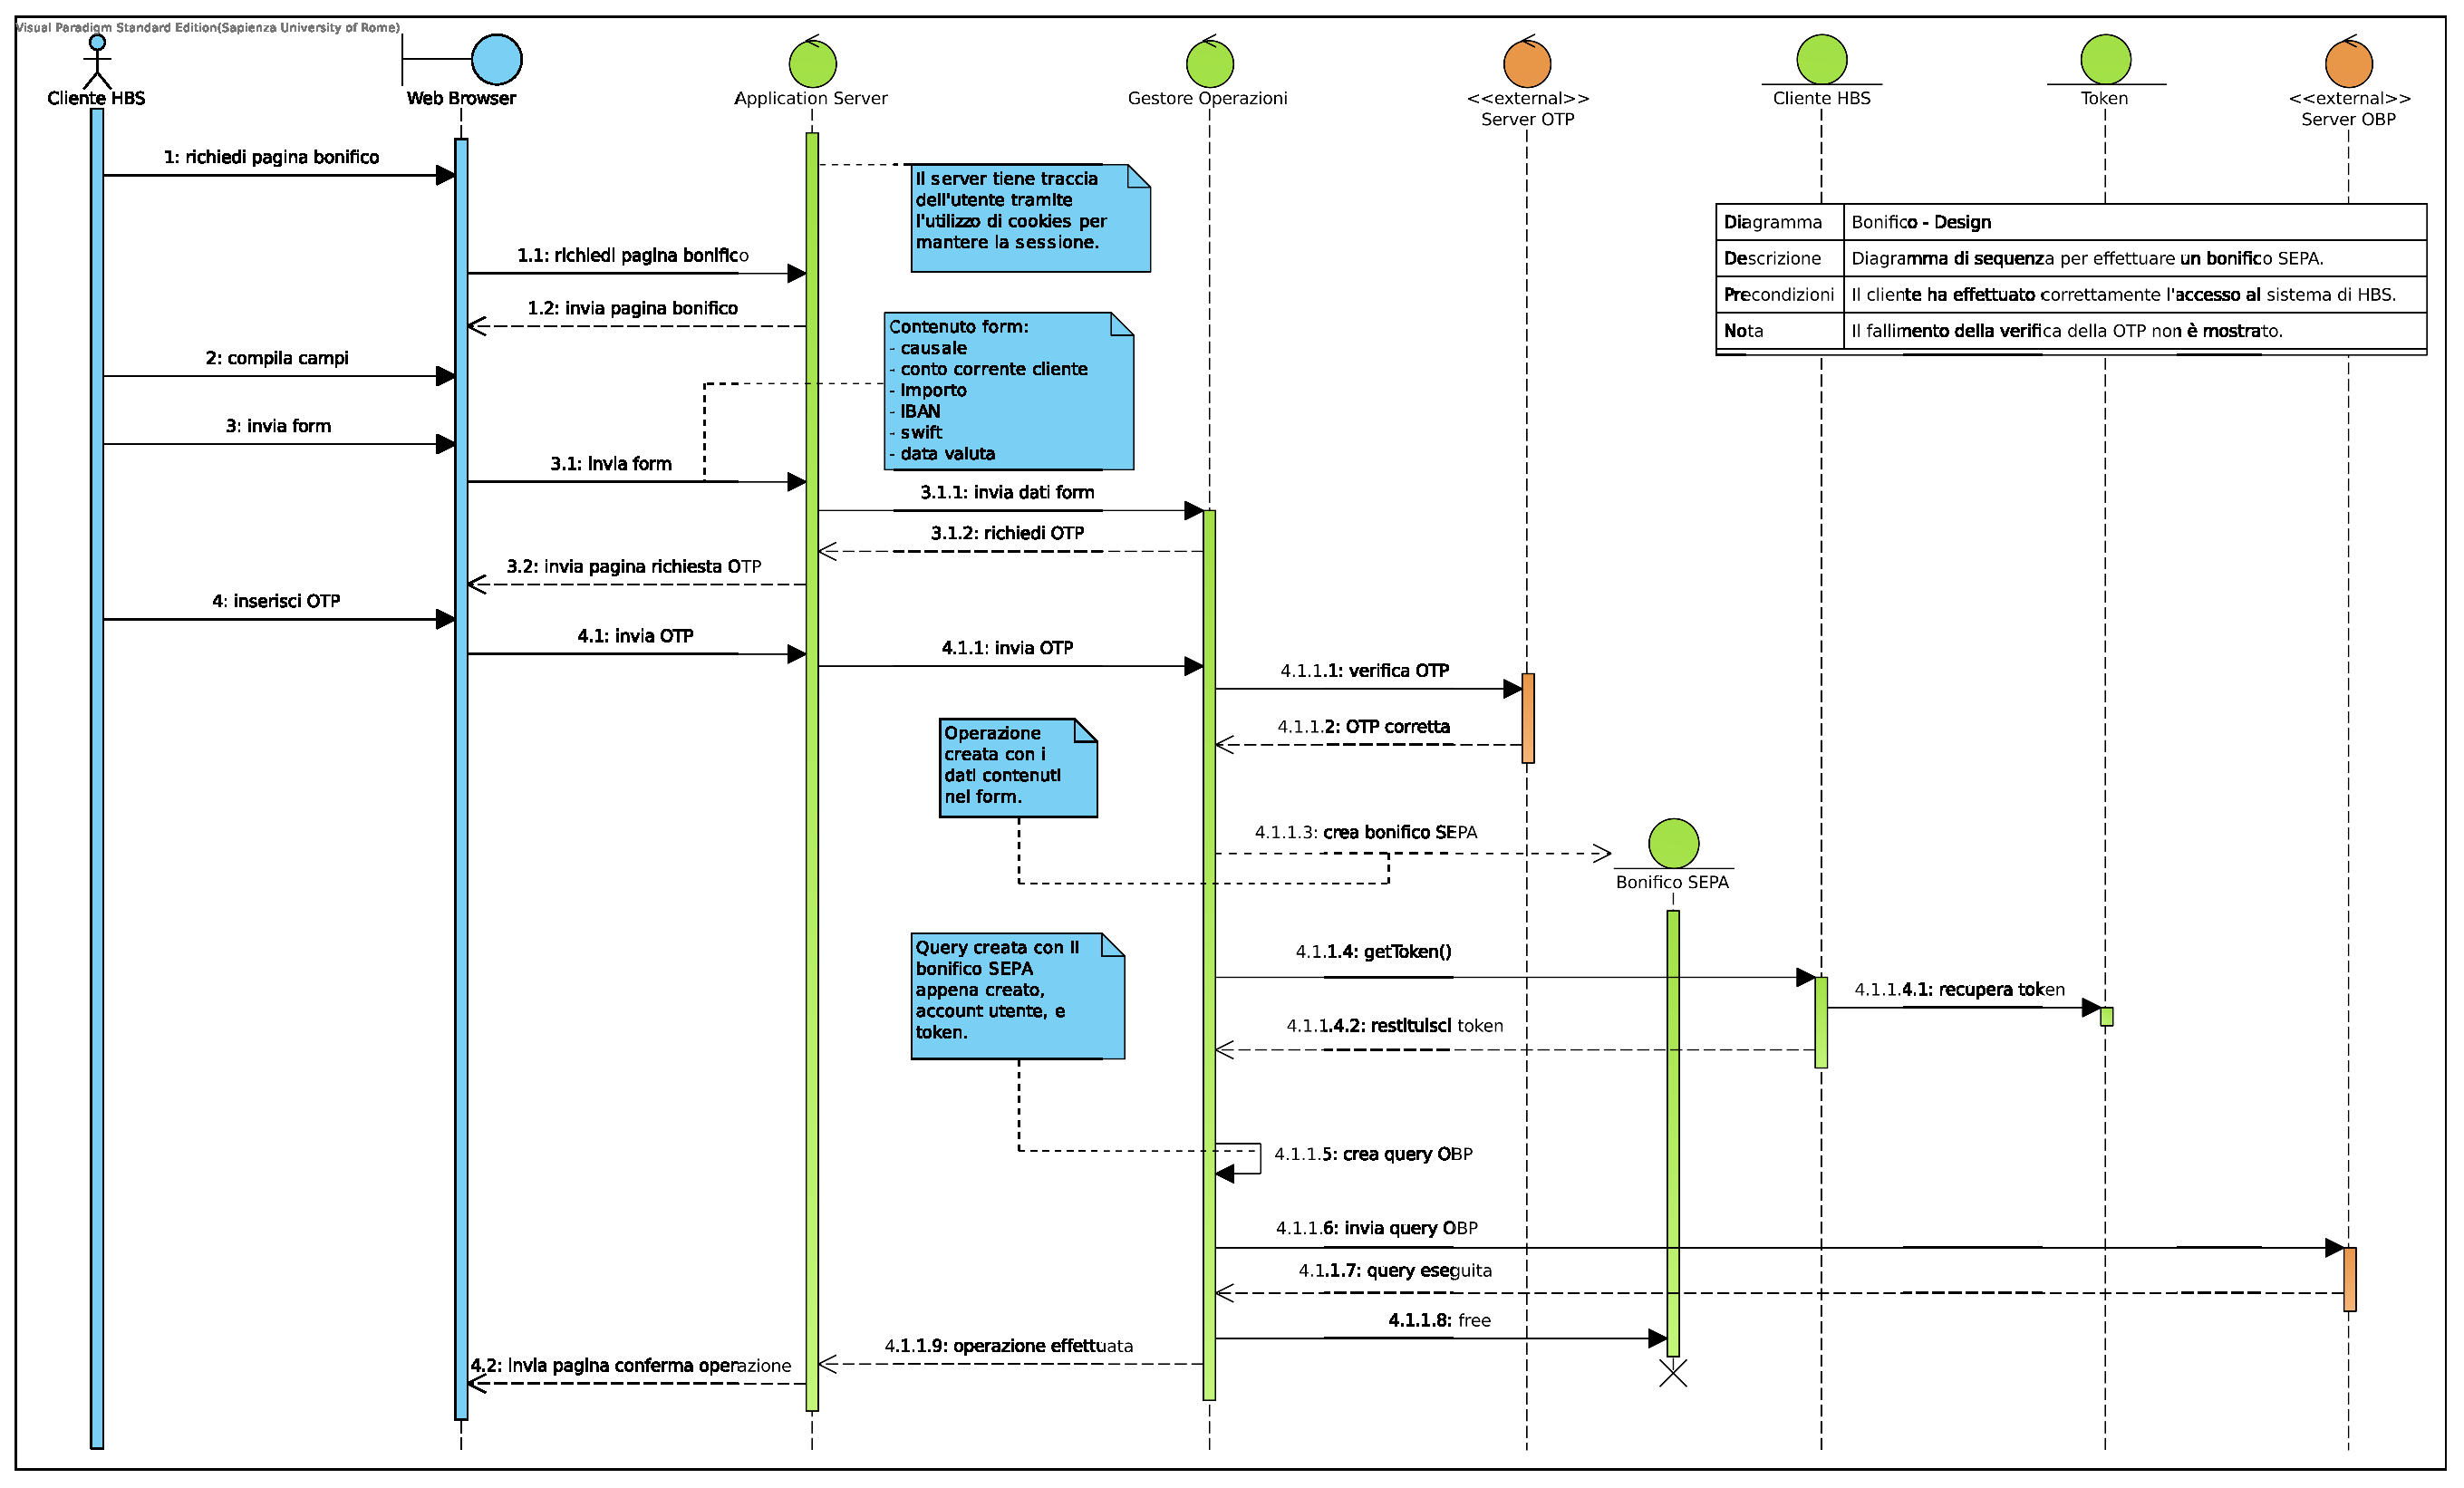
\includegraphics[width=\textheight, angle=90]{Images/Bonifico_-_Design.eps}
    \caption{Diagramma di sequenza relativo all'invio di un bonifico SEPA.}
    \label{fig:sequenza:bonifico-sepa}
\end{figure*}


